\documentclass{article}

\usepackage{amsmath}
\usepackage{upgreek}
\usepackage{dsfont}
\usepackage{mdframed}
%margin package
\usepackage[margin=1in,includefoot]{geometry}
%graphics packages
\usepackage{graphicx}
\usepackage{float}
%pseudocode packages
\usepackage{amsmath}
\usepackage{algorithm}
\usepackage[noend]{algpseudocode}
\usepackage{listings}


\begin{document}

\begin{enumerate}

%% PROBLEM 37 %%%%%%%%%%%%%%%%%%%%%%%%%%%%%%%%%%%%%%%%%%%%%%%%%%%%%%%%%%%%%%%%%%%%%%%%%%%%%%%%%%
\item Construir un ejemplo que muestre que la convergencia del m\'etodo de Jacobi no implica la convergencia del m\'etodo de Gauss-Seidel.
\\
\\
Para esto, usemos una matriz de $3x3$ del tipo :
\begin{gather*}
A = 
\begin{bmatrix}
	     1 	 & x_{4} &  x_{5} \\
	   x_{1} &   1   &  x_{6} \\
	   x_{2} & x_{3} & 	  1  
\end{bmatrix}
\end{gather*}
En funci\'on de esta matriz tenemos que las matrices de Jacobi y Gauss-Seidel son :
\begin{gather*}
B_{J} = 
\begin{bmatrix}
		0	 &  -x_{4}	& -x_{5} \\
	  -x_{1} & 	   0	& -x_{6} \\
	  -x_{2} & 	-x_{3}  &    0
\end{bmatrix},
B_{GS} = 
\begin{bmatrix}
	0	&				x_{4}			&	x_{5} \\
    0	& 			-x_{1}x_{4}			& x_{6} - x_{1}x_{5} \\
    0	& -x_{2}x_{4} + x_{1}x_{3}x_{4} & x_{1}x_{3}x_{5} - x_{2}x_{5} - x_{3}x_{6}
\end{bmatrix}
\end{gather*}
\\
Al obtener los autovalores de estas matrices, tendremos que los polinomios caracter\'isticos respectivos ser\'an los siguientes :
\begin{gather*}
P_{GS}(\lambda) = \lambda ( \lambda^{2} + \lambda ( x_{1}x_{3}x_{5} - x_{1}x_{4} - x_{2}x_{5} - x_{3}x_{6} ) + x_{2}x_{4}x_{6} ) = 0 \\
P_{J}(\lambda) = \lambda^{3} - \lambda( x_{1}x_{4} + x_{2}x_{5} + x_{3}x_{6} ) + x_{1}x_{3}x_{5} + x_{2}x_{4}x_{6} = 0
\end{gather*}
\\
Usemos un script que nos permita poder obtener los valores de $x_{i}$ que hacen que la matriz de Jacobi tenga radio espectral $\rho(B_{J}) < 1$ y a su vez radio espectral para la matriz de Gauss-Seidel $\rho(B_{GS}) > 1$. El script se muestra a continuaci\'on.
\\
\lstset{language=Python}
\begin{lstlisting}[frame=single]
import numpy as np

MIN = -3.0
STEP = 1.0
MAX = 3.0
N = int( ( MAX - MIN ) / STEP )

x1_set = [ MIN + STEP * q for q in range( N ) ]
x2_set = [ MIN + STEP * q for q in range( N ) ]
x3_set = [ MIN + STEP * q for q in range( N ) ]
x4_set = [ MIN + STEP * q for q in range( N ) ]
x5_set = [ MIN + STEP * q for q in range( N ) ]
x6_set = [ MIN + STEP * q for q in range( N ) ]

def getSpectralRadius_Gauss( x1, x2, x3, x4, x5, x6 ) :
    coeffs = [1, 
              x1 * x3 * x5 - x1 * x4 - x2 * x5 - x3 * x6,
              x2 * x4 * x6]

    leigs = np.roots( coeffs )
    maxnorm = np.abs( leigs[0] )
    for q in range( 1, len( leigs ) ) :
        _norm = np.absolute( leigs[q] )
        if ( _norm > maxnorm ) :
            maxnorm = _norm
    return maxnorm

def getSpectralRadius_Jacobi( x1, x2, x3, x4, x5, x6 ) :
    coeffs = [1,
              0, 
              -( x1 * x4 + x2 * x5 + x3 * x6 ),
              x1 * x3 * x5 + x2 * x4 * x6]

    leigs = np.roots( coeffs )
    maxnorm = np.abs( leigs[0] )
    for q in range( 1, len( leigs ) ) :
        _norm = np.absolute( leigs[q] )
        if ( _norm > maxnorm ) :
            maxnorm = _norm
    return maxnorm

cases = []

for x1 in x1_set :
    for x2 in x2_set :
        for x3 in x3_set :
            for x4 in x4_set :
                for x5 in x5_set :
                    for x6 in x6_set :
                        _sr_j = getSpectralRadius_Jacobi( x1, x2, x3, x4, x5, x6 )
                        _sr_g = getSpectralRadius_Gauss( x1, x2, x3, x4, x5, x6 )
                        
                        if ( _sr_j < 1 and _sr_g > 1 ) :
                            print '_sr_j: ' , _sr_j
                            print '_sr_g: ' , _sr_g
                            cases.append( [x1,x2,x3,x4,x5,x6] )

for case in cases :
    print 'case: ', case
\end{lstlisting}
Haciendo la b\'usqueda con ayuda del script vemos que los casos que cumplen son de la forma :

\begin{figure}[H]
	\centering
	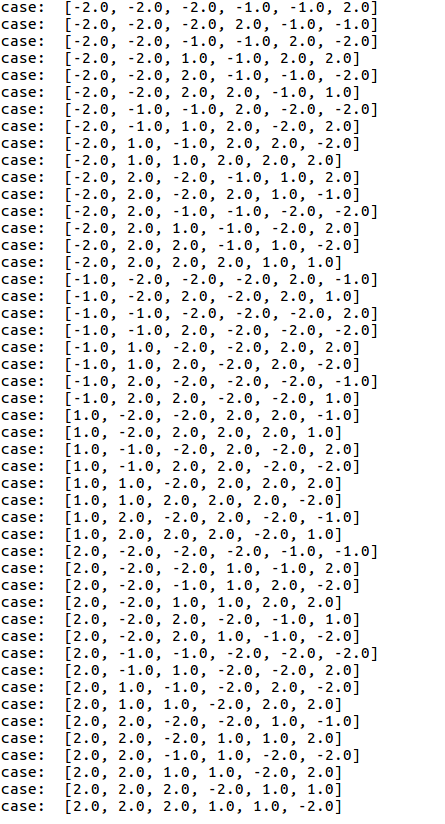
\includegraphics[scale=0.5]{/home/wilsan/Documents/wilbert/cs_master/courses/term1/numerical_linear_algebra/repo/hw/imgs/cases_prob_37.png}
	\caption{Casos con $\rho(j) < 1$ y $\rho(gs) > 1$}
	\label{fig:img_pecc}
\end{figure}
Las matrices para $x_{1}=-2,x_{2}=-2,x_{3}=-2,x_{4}=-1,x_{5}=-1,x_{6}=2$ :
\begin{gather*}
B_{J} = 
\begin{bmatrix}
		0 & 1 &  1 \\
	    2 & 0 & -2 \\
	    2 & 2 &  0
\end{bmatrix},
B_{GS} = 
\begin{bmatrix}
	0 & 1 &	1 \\
    0 & 2 & 0 \\
    0 & 6 & 2
\end{bmatrix}
\end{gather*}
%% PROBLEM 2 %%%%%%%%%%%%%%%%%%%%%%%%%%%%%%%%%%%%%%%%%%%%%%%%%%%%%%%%%%%%%%%%%%%%%%%%%%%%%%%%%%%
\item Sea $A \in R^{nxn} $ una matriz estrictamente diagonal dominante por filas. Muestre que el m\'etodo de Gauss-Seidel para la soluci\'on de $Ax = b$ es convergente.
\\
Para esto, bastar\'a probar que el radio espectral de la matriz de Gauss-Seidel es menor que 1, osea $\rho(B_{gs}) < 1$.
Partamos de que $\lambda$ sea un valor propio de $B_{gs}$. Entonces se debe cumplir:
\begin{gather*}
B_{gs}x = \lambda x
\end{gather*}
Donde $x$ es el vector propio asociado a $\lambda$. Adem\'as, tenemos que la matriz de Gauss-Seidel se expresa de la siguiente forma:
\begin{gather*}
B_{gs} = -( D + L )^{-1}U
\end{gather*}
Por lo que al usar la definici\'on de valor propio, tendremos lo siguiente:
\begin{gather*}
-Ux = \lambda ( D + L )x
\end{gather*}
Si analizamos la expresi\'on anterior por filas, tenemos para la fila $i$ la siguiente igualdad :
\begin{gather*}
-\sum_{j=i+1}^{n}a_{ij}x_{j} = \lambda ( \sum_{j=1}^{i}a_{ij}x_{j} ) = \lambda ( \sum_{j=1}^{i-1}a_{ij}x_{j} + a_{ii}x_{i}) \\
\rightarrow \lambda a_{ii}x_{i} = -\lambda \sum_{j=1}^{i-1}a_{ij}x_{j} - \sum_{j=i+1}^{n}a_{ij}x_{j}
\end{gather*}
Sea $x_{k}$ el mayor elemento en valor absoluto de $x$. Adem\'as, si $x$ es un valor propio, entonces $\frac{x}{s}$ tambi\'en es un valor propio ( escalar el vector propio sigue generando un vector propio ), por lo que podemos escoger $x$ que sea un vector propio escalado tal que la mayor componente sea 1, osea $\vert x_{k} \vert = 1$. Usando esto en la expresi\'on anteior tenemos que, para la fila $k$ :
\begin{gather*}
\lambda a_{kk} x_{k} = -\lambda \sum_{j=1}^{k-1}a_{kj}x_{j} - \sum_{j=k+1}^{n}a_{kj}x_{j}
\end{gather*}
Usando que $\vert x_{k} \vert =1$ es la mayor componente en valor absoluto, tenemos que :
\begin{gather*}
\vert \lambda \vert \vert a_{kk} \vert \vert x_{k} \vert \leq 
	\vert \lambda \vert \sum_{j=1}^{k-1} \vert a_{kj} \vert \vert x_{j} \vert +
	\sum_{j=k+1}^{n} \vert a_{kj} \vert \vert x_{j} \vert \\
\rightarrow
\vert \lambda \vert \vert a_{kk} \vert \leq 
	\vert \lambda \vert \sum_{j=1}^{k-1} \vert a_{kj} \vert +
	\sum_{j=k+1}^{n} \vert a_{kj} \vert \\
\vert \lambda \vert ( \vert a_{kk} \vert - \sum_{j=1}^{k-1} \vert a_{kj} \vert ) \leq 
	\sum_{j=k+1}^{n} \vert a_{kj} \vert \\	
\end{gather*}
Dado que $A$ es diagonal dominante, tenemos que :
\begin{gather*}
\vert a_{kk} \vert > \sum_{j=1,j \neq k}^{n} \vert a_{kj} \vert =
	\sum_{j=1}^{k-1}\vert a_{kj} \vert + \sum_{j=k+1}^{n} \vert a_{kj} \vert \\
\rightarrow
\vert a_{kk} \vert - \sum_{j=1}^{k-1}\vert a_{kj} \vert > \sum_{j=k+1}^{n} \vert a_{kj} \vert
\end{gather*}
Reemplazando esto en la expresi\'on anterior tendremos que $\vert \lambda \vert < 1 $, para cualquier $\lambda$ autovalor de la matriz de Gauss-Seidel, en particular el de mayor valor absoluto, por lo que el radio espectral de la matriz de Gauss-Seidel ser\'a menor que 1 ( $\rho(B_{GS}) < 1$ ), lo cu\'al demuestra que el m\'etodo converger\'a a la soluci\'on.
%% PROBLEM 2 %%%%%%%%%%%%%%%%%%%%%%%%%%%%%%%%%%%%%%%%%%%%%%%%%%%%%%%%%%%%%%%%%%%%%%%%%%%%%%%%%%%
\item Probar la recurrencia siguiente, que se obtiene del m\'etodo del gradiente conjugado :
\begin{gather*}
Ar_{k} = -\frac{1}{\alpha_{k}}r_{k+1} + ( \frac{1}{\alpha_{k}} - \frac{\beta_{k-1}}{\alpha_{k-1}} )r_{k} + \frac{\beta_{k-1}}{\alpha_{k-1}}r_{k-1}
\end{gather*}
\\
Para obtener la recurrencia empecemos por la expresi\'on recursiva del residual $r_{k}$ :
\begin{gather*}
r_{k+1} = r_{k} - \alpha_{k} A p_{k}
\end{gather*}
De la expresi\'on para la direcci\'on conjugada $p_{k}$ :
\begin{gather*}
p_{k} = r_{k} - \beta_{k} p_{k-1}
\end{gather*}
Reemplazando en la primera expresi\'on tenemos que :
\begin{gather*}
r_{k+1} = r_{k} - \alpha_{k} A ( r_{k} - \beta_{k-1} p_{k-1} ) \\
\rightarrow
\alpha_{k} A r_{k} = -r_{k+1} + r_{k} + \alpha_{k} \beta_{k-1} A p_{k-1} \\
\rightarrow
A r_{k} = -\frac{1}{\alpha_{k}} r_{k+1} + \frac{1}{\alpha_{k}} r_{k} + \beta_{k-1} A p_{k-1} \\
\end{gather*}
De la recurrencia para el residual, podemos tener lo siguiente :
\begin{gather*}
r_{k} = r_{k-1} - \alpha_{k-1} A p_{k-1} \\
\rightarrow
A p_{k-1} = \frac{ r_{k-1} - r_{k} }{\alpha_{k}}
\end{gather*}
Reemplazando en la expresi\'on anterior, tenemos :
\begin{gather*}
A r_{k} = -\frac{1}{\alpha_{k}} r_{k+1} + \frac{1}{\alpha_{k}} r_{k} + \beta_{k-1} ( \frac{r_{k-1} - r_{k}}{\alpha_{k-1}} ) \\
\rightarrow
A r_{k} = -\frac{1}{\alpha_{k}} r_{k+1} + 
			( \frac{1}{\alpha_{k}} - \frac{\beta_{k-1}}{\alpha_{k-1}} ) r_{k} +
			\frac{\beta_{k-1}}{\alpha_{k-1}} r_{k-1}
\end{gather*}
La cu\'al es la recurrencia que queriamos obtener.
\end{enumerate}
\end{document}